\documentclass[UTF8,a4paper,8pt]{ctexart} 

\usepackage{graphicx}%学习插入图
\usepackage{verbatim}%学习注释多行
\usepackage{booktabs}%表格
\usepackage{geometry}%图片
\usepackage{amsmath} 
\usepackage{amssymb}
\usepackage{listings}%代码
\usepackage{xcolor}  %颜色
\usepackage{enumitem}%列表格式
\CTEXsetup[format+={\flushleft}]{section}


\geometry{left=1.6cm,right=1.8cm,top=2cm,bottom=1.7cm} %设置文章宽度

\pagestyle{plain} 		  %设置页面布局
\author{郑华}
\title{Win 编程}
%代码效果定义
\definecolor{codegreen}{rgb}{0,0.6,0}
\definecolor{codegray}{rgb}{0.5,0.5,0.5}
\definecolor{codepurple}{rgb}{0.58,0,0.82}
\definecolor{backcolour}{rgb}{0.95,0.95,0.92}

\lstdefinestyle{mystyle}{
	backgroundcolor=\color{backcolour},   
	commentstyle=\color{codegreen},
	keywordstyle=\color{magenta},
	numberstyle=\tiny\color{codegray},
	stringstyle=\color{codepurple},
	basicstyle=\footnotesize,
	breakatwhitespace=false,         
	breaklines=true,                 
	captionpos=b,                    
	keepspaces=true,                 
	%numbers=left,                    
	%numbersep=5pt,                  
	showspaces=false,                
	showstringspaces=false,
	showtabs=false,                  
	tabsize=2
}
\lstset{style=mystyle, escapeinside=``}

\begin{document}          %正文排版开始
	\maketitle

   
\section{新数据类型}主要目的是 容易标识 变量的功能,其实现类似于 宏定义“Define UINT  unsigned int”
     \begin{itemize}
     	\item - MSG:消息类型
     	\item - HWND:句柄,就是一个资源标识,类似与指针,通过其找到对应的资源
     	\item - UNIT:unsigned int
     	\item - WM\_: windows message 标识前缀 
     	\item - WPARAM 、LPARAM:附加消息
     	\item - DWORD: 32位的整数
     	\item - POINT: 点,位置类型,成员x、y
     \end{itemize}  
 	
\section{Windows 应用关系}	 

   	\paragraph {0.设计一个WinFrame的基本步骤}:
   	
		   	1- 设计一个窗口类
		   	
		   	  WNDCLASS  winClass; WNDCLASSEX
		   	  
		   	2- 注册窗口类
		   	
		   	  RegisterClass(\&winClass);
		   	  
		   	3- 创建窗口
		   	
		   	  hwnd = CreateWindow(...);
		   	  
		   	4- 显示和更新窗口
		   	
		   	  ShowWindow(hwnd,nCmdShow);
		 
		   	  UpdateWindow(hwnd);
		   	  
		   	5- 消息循环
		   	
		   	  while(GetMessage(\&msg,NULL,0,0))\{
		   	  	
		   	  	TranslateMessage(\&msg);
		   	  	
		   	  	DispatchMessage(\&msg);
		   	  	
		   	  \}
		   	  \subparagraph{在vs2010 中的创建}:
		   	  
		   	   1- 新建win32
		   	   
		       2- 选择windows Application
		       
		       3- 下一步 不用选择Empty工程,直接生成即可
 	\paragraph {1.WinMain 函数}
	 	: Windows 程序的入口函数, WINAPI是一个Windows定义的宏,将使系统以特定于Windows 
 		
 	\paragraph {2.窗口类}
	 	:利用\textbf{结构体WNDCLASS 进行定义窗口样式},如图\ref{fig:winClass} ,消息处理函数的函数指针lpfnWndoroc,背景画刷hbrBac = (HBBRUSH)GetStockObject(颜色),菜单,窗口名等,然后利用Register(\&winclass)进行注册,然后利用CreateWindow创建,并利用句柄进行保存存或指向它,如图\ref{fig:createWindow} 
    	\begin{figure}
		   \begin{center}
			\begin{minipage}[H]{0.5\textwidth}
			 \centering
				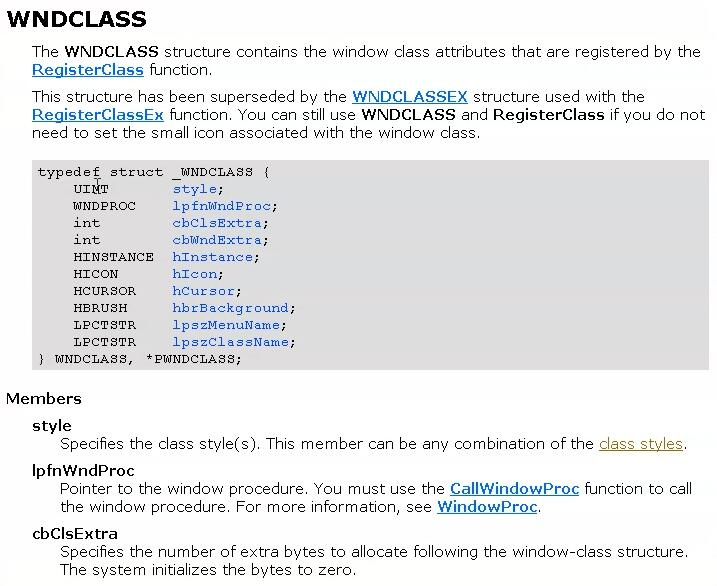
\includegraphics[angle=0,width=8cm,height=5.6cm]{wndClass.jpg}%就在前面括号中写图片名
				\caption{wndClass图}
				\label{fig:winClass}
		     \end{minipage}%
			\begin{minipage}[H]{0.5\textwidth} 
			 \centering
			    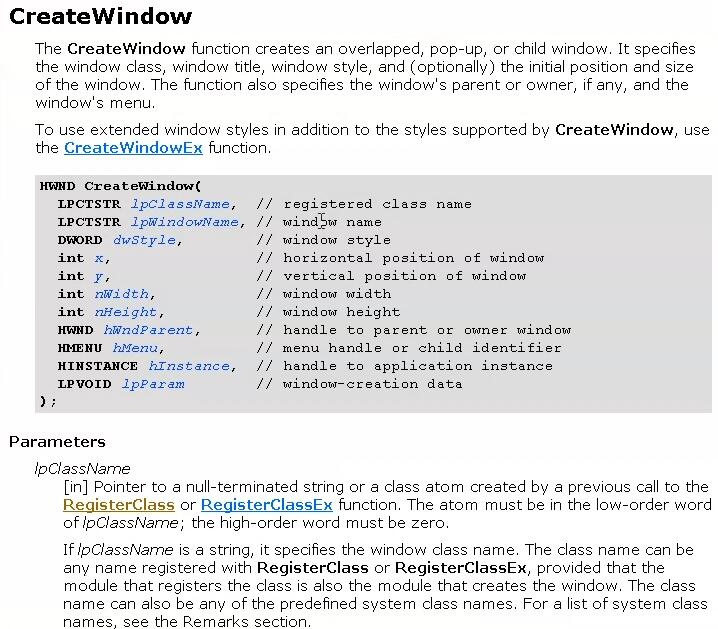
\includegraphics[angle=0,width=8cm,height=5.6cm]{createWindow.jpg}
			    \caption{createWindow图 }
				\label{fig:createWindow}
			\end{minipage}
		\end{center}
	\end{figure} 	
 		
    \paragraph {3.退出} 
        利用PostQuitMessage(0) 使程序结束
    
    \paragraph{4.示例代码}
	    \begin{lstlisting}[language=C++]
	       #include<Windows.h>  

	       LRESULT CALLBACK WndProc( HWND hwnd, UINT message, WPARAM wParam, LPARAM lParam );  

	       int WINAPI wWinMain( HINSTANCE hInstance, HINSTANCE prevInstance, LPWSTR cmdLine,int cmdShow )  
	       {  
	       UNREFERENCED_PARAMETER( prevInstance );  
	       UNREFERENCED_PARAMETER( cmdLine );  
	       
	       WNDCLASSEX wndClass = { 0 };  
	       wndClass.cbSize = sizeof( WNDCLASSEX ) ;  
	       wndClass.style = CS_HREDRAW | CS_VREDRAW;  
	       wndClass.lpfnWndProc = WndProc;  
	       wndClass.hInstance = hInstance;  
	       wndClass.hCursor = LoadCursor( NULL, IDC_ARROW);  
	       wndClass.hbrBackground = ( HBRUSH )(COLOR_WINDOW + 1 );  
	       wndClass.lpszMenuName = NULL;  
	       wndClass.lpszClassName = "DIRECTX11BookWindowClass";  
	       
	       if( !RegisterClassEx( &wndClass ) )  
	       return -1;  
	       
	       RECT rc = { 0, 0, 640, 480 };  
	       AdjustWindowRect( &rc,WS_OVERLAPPEDWINDOW, FALSE );  
	       
	       HWND hwnd = CreateWindowA( "DIRECTX11BookWindowClass","Blank Win32 Window",  
	       WS_OVERLAPPEDWINDOW, CW_USEDEFAULT,CW_USEDEFAULT, rc.right - rc.left,  
	       rc.bottom - rc.top, NULL, NULL,hInstance, NULL );  
	       
	       if( !hwnd )  
	       return -1;  
	       
	       ShowWindow( hwnd, cmdShow );  
	       

	       MSG msg = { 0 };  
	       
	       while( msg.message != WM_QUIT )  
	       {  
	       if( PeekMessage( &msg, 0, 0, 0,PM_REMOVE ) )  
	       {  
	       TranslateMessage( &msg );  
	       DispatchMessage( &msg );  
	       }  
	       else  
	       {  

	       }  
	       }  
	       
	       
	       return static_cast<int>( msg.wParam);  
	       }  
	       
	       
	       
	       
	       LRESULT CALLBACK WndProc( HWND hwnd, UINT message, WPARAM wParam, LPARAM lParam )  
	       {  
	       PAINTSTRUCT paintStruct;  
	       HDC hDC;  
	       
	       switch( message )  
	       {  
	       case WM_PAINT:  
	       hDC = BeginPaint( hwnd,&paintStruct );  
	       EndPaint( hwnd, &paintStruct);  
	       break;  
	       
	       case WM_DESTROY:  
	       PostQuitMessage( 0 );  
	       break;  
	       
	       default:  
	       return DefWindowProc( hwnd,message, wParam, lParam );  
	       }  
	       
	       return 0;  
	       }  
	    \end{lstlisting}
	 
 \section{消息映射}
  
	  \paragraph{1- 头文件要做的}:
	      
	      %对应消息的处理函数
	      afx\_msg void OnPaint();     %ON_WM_PAINT() 对应的消息处理函数
	      
	      DECLARE\_MESSAGE\_MAP();
	      
	  \paragraph{2- 源文件要做的}:
	  
	      BEGIN\_MESSAGE\_MAP()
	       
	       %需要自己处理的消息
	       ON\_WM\_PAINT()          %ON_WM_PAINT() 对应的消息处理函数为 afx_msg void OnPaint()
	       
	       ON\_WM\_LBUTTONDOWN()    %ON_WM_LBUTTONDOWN() 对应的消息处理函数为 afx_msg void OnLButtonDown(UINT nFlags, CPoint point)
	      
	      END\_MESSAGE\_MAP()
	      
	  \paragraph{3- 右键类点击属性进行添加消息}
 
 
 \section{字符集 与 TEXT宏}
  
	  8位ANSI字符集
	  
	  16位unicode 字符集 - 宽字符集
	  
	  TEXT宏(\_T宏)
	  
	  TCHAR、TCHAR*、LPTSTR、LPCTSTR
	  
	  API 分ANSI 和 Unicode两个版本
  
	  \paragraph{1.ANSI 8位}:
	  
		  char szMsgA[256]  = "hello";
		  
		  strcat(szMsgA,"ss");
		  
		  ::MessageBoxA(NULL,szMsgA,"窗口名",MB\_OK);
	  
	  \paragraph{2.Unicode 16位}:
	   
		   wchar\_t szMsgW[256] = L"hello";
		   
		   宽型字符串直接 添加L
		   
		   lstrcatW(szMsgW,L", unicode");
		   
		   ::MessageBoxW(NULL, szMsgW,L"hello",MB\_OK);
	   
	   \paragraph{3.自适应类型}:
		   
		   TCHAR szMsgT[256] = TEXT("Hello");
		   
		   LPTSTR st = TEXT("hello");
		   
		   LPCTSTR sct = TEXT("hello");
		   
		   \_tcscat(szMsgT,TEXT(",TCHAR"));
		   
		   ::MessageBox(NULL,, szMsgT,TEXT("hello"),MB\_OK)
   
   
   \section{常规空MFC 的建立}
	   1.Visual C++ - General
	   
	   2.Empty Project
	   
	   3.右键项目--属性
	   
	   4.配置MFC的使用dll
	   
	   5.配置字符集unicode
   
   
  \section{MFC 设备绘图类}:
	    \paragraph{1.windows GDI}:
	    
		     \textbf{1- GDI}
		     
		     \textbf{2- DC}
		            
		     最后的一个点不画【左闭右开】
	    \paragraph{2.MFC绘图类}:
	    
		    \textbf{1- CDC}
		     
		    \textbf{2- CPaintDC}
		     
		     (1)CPaintDC类是CDC类的一个派生类,该类一般用在响应WM\_PAINT消息的函数OnPaint()中。
		     
		     (2)WM\_PAINT消息是当窗口的某个区域需要重画时激发的窗口消息。当程序中的消息循环接到WM\_PAINT消息时就自动调用消息处理函数OnPaint(),如果在OnPaint函数内定义了CPaintDC类的对象,通过这个类对象就可以使用CDC类的成员函数完成视图客户区中的图形绘制操作。
		     
		     (3)CPaintDC用于响应窗口重绘消息(WM\_PAINT)时的绘图输出。CPaintDC在构造函数中调用BeginPaint()取得设备上下文,在析构函数中调用EndPaint()释放设备上下文。EndPaint()除了释放设备上下文外,还负责从消息队列中清除WM\_PAINT消息。因此,在处理窗口重画时,必须使用CPaintDC,否则WM\_PAINT消息无法从消息队列中清除,将引起不断的窗口重画。\textbf{CPaintDC也只能用在WM\_PAINT消息处理之中。}
		     
		     \textbf{3- CClientDC}
		  
		       CClientDC类也是CDC类的派生类。\textbf{它只能在窗口的客户区(即窗口中除了边框、标题栏、菜单栏以及状态栏外的中间部分)中进行绘图},坐标点(0,0)通常指的是客户区的左上角。它的构造函数调用GegDC函数,而析构函数调用ReleaseDC函数。
		       CClientDC(客户区设备上下文)用于客户区的输出,它在构造函数中封装了GetDC(),在析构函数中封装了ReleaseDC()函数。一般在响应非窗口重画消息(如键盘输入时绘制文本、鼠标绘图)绘图时要用到它。用法是:
		  
		       CClientDC dc(this);//this一般指向本窗口或当前活动视图
		  
		       dc.TextOut(10,10,str,str.GetLength());
		  
			  //利用dc输出文本,如果是在CScrollView中使用,还要注意调用OnPrepareDC(\&dc)调整设备上下文的坐标。
		  
		    \textbf{4- CWindowDC}
		     
		     CWindowDC类也是CDC类的派生类。\textbf{其成员函数可以在窗口的客户区和非客户区(即窗口的边框、标题栏、菜单栏以及状态栏)中绘图,坐标点(0,0)是指整个屏幕的左上角。}同CClientDC类一样,它的构造函数调用GegDC函数,而析构函数调用ReleaseDC函数。
	     
	     \paragraph{3.绘图函数}:
	     
		     POINT points[5] = {10,10,  20,20,  30,30,  40,40,  50,50};
		     
		     dc.Polyline(points,5);
		     
		     贝塞尔曲线:
		     
		     dc.PolyBezier(points,4);
		     
		     矩形区域:
		     
		     CRect rect(左\_x,左\_y,右下\_x,右下\_y);
		     
		     画矩形:
		     
		     dc.Rectangle(rect);
		     
		     画椭圆:
		     
		     dc.Ellipse(rect);
		     
		     画弧线:截取椭圆
		     
		     dc.Arc(10,10,  200,100, 0,0,  80,200);
		     
		     画扇形:
		     
		     dc.Pie(rect,point1, point2);
		     
		     画弦:
		     
		     dc.Chord(rect,point1, point2);
	     \paragraph{4.画笔与画刷}:
	     
		\textbf{使用画笔--方式1:}
		     
		     CPen pen(PS\_SOLID,6,RGB(255,0,0 ));
		     
		     PS\_DASH :虚线
		     
		     PS\_DOT : 点线
		     
		     dc.SelectObject(\&pen);
	     
		\textbf{使用画笔--方式2:}
		     
		     CPen pen3;
		     
		     LOGPEN lp;
		     
		     lp.lopnStyle = PS\_DASHDOT;
		     
		     lp.lopnWidth.x = 1;
		     
		     lp.lopnColor = RGB(0,0,255);
		     
		     pen3.CreatePenIndirect(\&lp);
		     
		     dc.SelectObject(\&pen3);
		     
		\textbf{使用画刷:背景色,填充色}
		     
		     CBrush brush(RGB(0,0,255));
		     
		     或brush(HS\_DIAGCROSS 斜网格,RGB(0,255,255));
		     
		     HS\_BDIAGONAL : 斜线
		
		     HS\_CROSS: 正网格
		     
		     HS\_FDIAGONAL: 反斜线
		     
		     HS\_HORIZONTAL: 正斜线
		          
		     dc.SelectObject(\&brush);
		       
		     dc.Rectangle(...);
	     
	     \paragraph{5.画文本}:
	     
		     \textbf{1- dc.DrawText:}
		     
		     dc.DrawText(TEXT("Hello"),-1,\&rect,DT\_SINGLELINE | DT\_CENTER | DT\_VCENTER);
		     
		     \textbf{2- dc.TextOut}
		     
		     dc.TextOut(100,100,TEXT("Hello"));
		     
		     \textbf{3- 字体:}
		     
		     \textbf{方式1:}
		     
		     CFont font;
		     
		     font.CreatePointFont(72*10,TEXT("Arial"));
		     
		     dc.SelectObject(\&font);
		     
		     \textbf{方式2:}
		     
		     LOGFONT lf;
		     
		     ::ZeroMemory(\&lf,sizeof(lf));
		     
		     lf.lfHeight = 120;
		     
		     lf.lfWeight = FW\_BOLD;
		     
		     lf.lfItalic = TRUE;
		     
		     ::lstrcpy(lf.lfFaceName, TEXT("Times New Roman"));
		     
		     CFont font\_Indirect;
		     
		     font\_Indirect.CreatePointFontIndirect(\&lf);
		     
		     偏移:rect.Offset
		     
		     \textbf{旋转:}
		     
		     lf.lfEscapement = 45 *10;
		     
		     lf.lfOrientation = 45 *10;
	     
	     \paragraph{6.备用对象 画笔画刷}:
	     
		     \textbf{选择备用的画笔}:
		     
		     dc.SelectStockObject(NULL\_PEN); 
		     
		     \textbf{选择备用的画刷}:
		     
		     dc.SelectStockObject(LTGRAY\_BRUSH);
		     
		     dc.SetMapMode(MM\_LOENGLISH);// 将坐标系转换为 数学 类型,但是左上角还为0,0
		     
		     dc.SetTextAlign(TA\_CENTER | TA\_BOTTOM); //文字的对齐模式
		     
		     dc.SetBkMode(TRANSPARENT); //设置透明     
	     
	     \paragraph{7.win32 画图不更新}
		     http://zhidao.baidu.com/link?url=BxIG\_kklq269UNNlR1HAAIk9fGlL2HtallG4\_zSSoRGOrRr3cnJ\_FXpTToyigOpDGrsL1JV1gdU3PIGmFx4xIa
	     
		     要设置失效区域
     
  \end{document} 
 		    